\documentclass[11pt]{article}
\usepackage{newcent}
\usepackage[english]{babel}
\usepackage[letterpaper]{geometry}
\usepackage{graphicx}

\def\cmd#1#2{\noindent {\bf #1} #2\par}
\def\expl#1{\kern-8pt\begin{itemize}\item[]#1\end{itemize}}
\def\cref#1{{\bf #1}}
\def\bar{{$|$}}
\def\nyi{{\par\bf\itshape Not yet implemented.}}
\def\matlab#1#2{{\bf #1}: #2\par}

\begin{document}
\begin{centering}
\noindent{\Large\bf Using QPlot as a stand-along program}\medskip

\noindent{\large\bf Daniel Wagenaar, 2014}\bigskip

\end{centering}

{\noindent\scriptsize\bf  Copyright (c) ~2014 ~Daniel A. Wagenaar
  
\noindent Permission is granted to copy, distribute and/or modify this document
under the terms of the GNU Free Documentation License, Version 1.3 or
any later version published by the Free Software Foundation; with no
Invariant Sections, no Front-Cover Texts, and no Back-Cover Texts.  A
copy of the license may be downloaded from
http://www.gnu.org/copyleft/fdl.html.}\bigskip


\noindent For most users, it will be much more convenient to use QPlot from
within Octave or Matlab. However, in certain situations, such as when
producing a large number of graphs in an automated fashion, or when
implementing a shell around QPlot for another computation environment
or programming language, it may be advantageous to use QPlot
directly. This document briefly describes how to do that.

\section{User interface}

QPlot can be run on the command line, like this:
\begin{quotation}
qplot \emph{source} \emph{output}
\end{quotation}
 where \emph{source} is a file with commands and
\emph{output} can specify either pdf, svg, png, or tiff output. Output
can also be a postscript (.ps) file, in which case a single full page
is produced with the graph in the middle and crop marks around
it. Output to eps is not directly supported, but ``pdftoeps -eps -level3'' can
be used as a postprocessor.

QPlot can also be run interactively, like this:
\begin{quotation}
qplot \emph{source}
\end{quotation}
 In that case, graphics are rendered in a window. Keys ``+''
and ``-'' zoom in and out, ``0'' scales to fit, ``1'' scales to
100\%. ``E'' resizes the window to fit the whole scene. ``G'' toggles
between white and gray borders. ``C'' enables or disables reporting
coordinates below the mouse pointer. ``Ctrl-Q'' quits. The graphics are
automatically rerendered if the \emph{source}
file changes on disk.



\section{Commands}
Optional arguments are given in parentheses. Vertical bars indicate
alternatives.\bigskip

\cmd{align}{left\bar{}right\bar{}center\bar{}top\bar{}bottom\bar{}middle\bar{}base}
\expl{Sets horizontal and/or vertical alignment for subsequent text.}

\cmd{area}{[ \emph{dx$_1$ dx$_2$ \ldots} ] [ \emph{dy$_1$ dy$_2$ \ldots}
]}
\expl{Draws a polygon, filled using the current brush. 
  \emph{dx$_i$} and \emph{dy$_i$} are specified in
  points and are relative to the position set by \cref{at}. Note that
  the ``['' and ``]'' are literal brackets that separate the x- and 
  y-coordinates. See also \cref{patch}.}

\cmd{at}{\emph{x} \emph{y}}
\cmd{at}{\emph{x} \emph{y} \emph{$\xi$} \emph{$\eta$}}
\cmd{at}{\emph{x} \emph{y} \emph{$\phi$}}
\cmd{at}{--}
\cmd{at}{\emph{x} \emph{y} \emph{ID}}
\cmd{at}{\emph{ID}}
\expl{Places subsequent text and lines at graph
    position (\emph{x}, \emph{y}). If (\emph{$\xi$}, \emph{$\eta$})
    are given, this specifies a rotation such that the baseline of the
    text is in the direction of the vector (\emph{$\xi$},
    \emph{$\eta$}). This vector is specified in data
    coordinates. Alternatively, a rotation may be specified as a
    direct (clockwise) angle $\phi$. Besides a numeric value, \emph{x}
    may be one of {``left''}, {``right''}, or {``center''} to place 
    relative to the
    bounding box of the last drawn object (or group, see
    \cref{group}), ``abs'' or ``absolute'' to revert to absolute
    placement in the horizontal direction, or a dash (``--'') to
    retain the previous anchor for
    the horizontal direction.  
    Likewise, \emph{y} may be one of {``top''}, {``bottom''},
    {``middle''}, ``abs'', ``absolute'', or a dash. ``at --''
    reverts to absolute placement (i.e., relative to the top left of the
    current panel)
    in both horizontal and vertical directions. \cref{at} may also be
    used to mark a location for later reference, as per the final two
    syntax forms.}

\cmd{brush}{(\emph{ID}) \emph{color}\bar{}none\bar{}\emph{opacity} \ldots}
\expl{Selects a brush by \emph{ID}, defines its color (or sets it to
  ``none''), and/or its \emph{opacity} (as a number between 0 and 1).}

\cmd{caligraph}{[ \emph{x$_1$ x$_2$ \ldots} ] 
                [ \emph{y$_1$ y$_2$ \ldots} ]
                [ \emph{w$_1$ w$_2$ \ldots} ]}
\expl{Draws a polyline of variable width.  \emph{x$_i$}
  and \emph{y$_i$} are specified in data coordinates. \emph{w$_i$}
  specify the line width (in points) at each vertex. (Thus, the length
  of the vector \emph{w} must match the length of \emph{x} and
  \emph{y}.) The line is rendered using the color of the current pen;
  dash patterns and join and cap styles are not respected.}

\cmd{figsize}{\emph{w} \emph{h}}
\expl{Sets the size of the figure to (\emph{w} x \emph{h})
  points. This should appear before any other commands.}

\cmd{font}{\emph{family} (bold) (italic) \emph{size}}
\expl{Selects a new font with a given family, point size, weight
  and/or slant.}

\cmd{garea}{( \emph{ptspec} ) \ldots}
\cmd{gline}{( \emph{ptspec} ) \ldots}
\expl{Ultraflexible polygon and line series drawing. 
  Each vertex is specified by a \emph{ptspec}, i.e., a sequence of one or
  more subcommands:\medskip\\
\mbox{}\kern10pt\begin{tabular}{lp{3.8in}}
{\bf absdata} \emph{x} \emph{y} & Absolute data coordinates \\
{\bf reldata} \emph{dx} \emph{dy} & Relative data coordinates \\
{\bf abspaper} \emph{x} \emph{y} & Absolute paper coordinates (in pt)\\
{\bf relpaper} \emph{dx} \emph{dy} & Relative data coordinates (in
               pt)\\
{\bf rotdata} $\xi$ $\eta$ & Rotate by atan2($\eta$, $\xi$) 
              in data space (this affects subsequent relative
              positioning) \\
{\bf rotpaper} $\phi$ & Rotate by $\phi$ radians (this affects
subsequent relative positioning) \\
{\bf retract} \emph{L} & Retract preceding and following segments by
              \emph{L} pt \\
{\bf retract} \emph{L$_1$} \emph{L$_2$} & Retract preceding and following
              segments by \emph{L$_1$} and \emph{L$_2$} pt
              respectively \\
{\bf at} \emph{ID} & Absolute paper coordinates of location set by \cref{at} \\              
{\bf atx} \emph{ID} & Absolute paper x-coordinate of location set by \cref{at} \\              
{\bf aty} \emph{ID} & Absolute paper y-coordinate of location set by \cref{at} \\              
\end{tabular}\medskip\\
For {\bf absdata} or {\bf abspaper}, either \emph{dx} or \emph{dy} may
be given as a dash (``-''), in which case the corresponding coordinate
is not affected. (To achieve the same for {\bf reldata} or {\bf
  relpaper}, just use zero.)
Note that the parentheses are literal, unlike in the rest of this manual, where
they designate optional parameters. For instance:\medskip\\
\mbox{}\kern15pt
       gline ( absdata 0 1 relpaper 5 0 ) ~ ( absdata 0 1 relpaper 0 5 )
\medskip\\
     draws a line from 5 pt to the right of the point (0,1) in the graph to
     5 pt above the point (1,0) on the graph.\\
(Note: The rather cumbersome syntax of \cref{gline} makes \cref{line}
     and \cref{plot} more attractive for general usage. The same
     applies to \cref{garea} versus \cref{area} and \cref{patch}.)
}


\cmd{group}{}
\cmd{endgroup}{}
\expl{Groups statements to accumulate bounding boxes for
  \cref{at}. \cref{endgroup} also restores pen, brush, alignment,
  font, and
  reference text to their states before the corresponding
  \cref{group}. Note that named pens and brushes changed inside a
  group are not restored. All groups must be closed before changing
  panels, else the group stack is cleared automatically and a warning
  message is issued. }

\cmd{hairline}{\emph{width}} \expl{Specifies a width for lines plotted
  with zero nominal width, in points. If \emph{width} is zero,
  hairlines are precisely one pixel wide in the output. This is very
  useful for raster output but not recommended for pdf or svg output,
  since the resulting file would become device dependent. The default
  is 0 for raster output (including interactive output), and 0.25 pt
  for svg/pdf/postscript.}

\cmd{image}{\emph{x y w h K} [ \emph{cdata} ]}
\expl{Renders an RGB image at given data location. \emph{cdata} is
  stored as (R,G,B) pixels in row order (unlike matlab's convention); 
   \emph{K} specifies
  the number of pixels per row. The length of \emph{cdata} must be an
  even multiple of 3\emph{K}. Values must be between 0 and 1.}

\cmd{line}{[ \emph{dx$_1$ dx$_2$ \ldots} ] [ \emph{dy$_1$ dy$_2$ \ldots} ]}
\expl{Draws a polyline. \emph{dx$_i$} and \emph{dy$_i$} are specified in
  points and are relative to the position set by \cref{at}. See also
  \cref{plot}.}

\cmd{mark}{[ \emph{x$_1$ x$_2$ \ldots} ] [ \emph{y$_1$ y$_2$ \ldots} ]}
\expl{Renders markers set by \cref{marker} at the given data
  coordinates.}

\cmd{marker}{\emph{size}\bar\emph{fill}\bar\emph{shape} \ldots) (open\bar{}solid\bar{}brush)
  ()
  \ldots}
\expl{Define a marker of the given \emph{size} in points and shape
  (one of
  ``circle'', ``square'', ``diamond'', ``left'', ``right'', ``up'',
  ``down'', ``penta'', ``hexa'', ``hbar'', ``vbar'', ``plus'', or ``cross'')
  for
  later use by \cref{mark} and \cref{pmark}. The \emph{fill} style
  specifies how the marks are rendered: An ``open'' mark  is 
  is outlined with the current pen and filled with white,  a ``solid'' is
  outlined with the current pen and filled with the pen color, and a  ``brush'' mark is outlined  with
  the current pen and filled with the current brush (which may be ``none''). The fill style
  has no effect on ``hbar'', ``vbar'', ``plus'', or ``cross'' marks.}

\cmd{panel}{\emph{ID}\bar--}
\cmd{panel}{\emph{ID x$_0$ y$_0$ w h}}
\expl{Defines a new panel with given ID to have its top left corner on
  paper position (\emph{x$_0$}, \emph{y$_0$}), in points, and size
  (\emph{w} x \emph{h}), in points. Or, reenters a previously defined
  panel. Or drops out to the top level. While drawing inside a panel,
  \cref{figsize} changes the size of the panel, and \cref{shrink}
  affects the panel rather than the figure as a whole. Also
  \cref{xaxis} and \cref{yaxis} affect the axes in the
  panel. Choices of pen, brush, font, etc., are not local to panels.}

\cmd{patch}{[ \emph{x$_1$ x$_2$ \ldots} ] [ \emph{y$_1$ y$_2$ \ldots} ]}
\expl{Draws a polygon, filled using the current brush. \emph{x$_i$}
  and \emph{y$_i$} are specified in data coordinates. See also \cref{area}.}

\cmd{pen}{(\emph{ID})
  \emph{color}\bar{}\emph{width}\bar{}%
  \emph{capstyle}\bar{}\emph{joinstyle}\bar{}%
  \emph{linestyle} \ldots}

\expl{Selects a pen by \emph{ID}, defines its color, its width (in
  points), its join style (one of ``miterjoin'', ``beveljoin'', or ``roundjoin''),
  its capstyle (one of ``flatcap'', ``squarecap'', or ``roundcap''), and/or its
  line style (one of ``solid'', ``dash'', ``dot'', or ``none'').
The word ``dash'' may optionally be followed by a single number or a
vector of numbers (in brackets) that defines the lengths of marks and
spaces (in points); the word ``dot'' may be followed by a single
number or a vector of numbers (in brackets) that defines the lengths
of the spaces between dots (in points). The default is
3~pts.
  Setting the color or width while the dash pattern is
  ``none'' automatically switches to ``solid.'' Any number of
  subcommands may be given on one line in any order. A \cref{pen}
  command without an \emph{ID} makes changes to the current pen but
  doesn't store the result as a named pen.}

\cmd{plot}{[ \emph{x$_1$ x$_2$ \ldots} ] [ \emph{y$_1$ y$_2$ \ldots}
]}
\expl{Draws a polyline. \emph{x$_i$}
  and \emph{y$_i$} are specified in data coordinates. See also
  \cref{line}.}

\cmd{pmark}{[ \emph{dx$_1$ dx$_2$ \ldots} ] [ \emph{dy$_1$ dy$_2$ \ldots} ]}
\expl{Renders markers set by \cmd{marker}. \emph{dx$_i$} and \emph{dy$_i$} are specified in
  points and are relative to the position set by \cref{at}. See also
  \cref{mark} and \cref{marker}.}

\cmd{reftext}{\emph{string}\bar{}--}
\expl{Sets or unsets a fixed text that will be used to calculate the
  ascent and descent of text for the ``bottom'' and ``top'' alignment
  modes.}

\cmd{sharelim}{(x|y) \emph{ID} \ldots}
\expl{Shrinks the x-axis and/or y-axis of the current panel and the
  named panel(s) so that they have a common scale. If the panels
  overlap horizontally (vertically) on the page, the x-axis (y-axis)
  are additionally aligned.}

\cmd{shrink}{(\emph{margin})}
\cmd{shrink}{\emph{margin} \emph{ratio}}
\cmd{shrink}{-- \emph{ratio}}
\expl{Shrinks the axes as necessary so that all graphics and text fits
  within the bounding box of the figure as defined by
  \cref{figsize}. Margin is specified in points. Optional \emph{ratio}
specifies the desired aspect ratio of y:x data units.}

\cmd{text}{\emph{dx} \emph{dy} \emph{string}}
\expl{Places the given text \emph{string} at the position (\emph{dx},
  \emph{dy}), specified in points relative to the anchor set by
  \cref{at}.\\ Underscores and hats make subscripts and superscripts
  (up to the next space). Slashes and asterisks make enclosed words
  appear in /italics/ and *bold*. Unicode is supported. The string
  must be enclosed in single or double quotes. Respects alignment
  options set by \cref{align}.}

\cmd{ctext}{\emph{dx} \emph{dy} \emph{string}}
\expl{Places the given text \emph{string} at the position (\emph{dx},
  \emph{dy}), specified in points relative to the position where the
  previous text rendering ended (rather than at the anchor set by
  \cref{at}). This ignores alignment options set by \cref{align}.}

\cmd{xlim}{\emph{x$_0$} \emph{x$_1$}}
\expl{Fixes the limits of the x-axis. (If no xlim is given for a panel, tight
  automatic axis limits apply.)}

\cmd{ylim}{\emph{y$_0$} \emph{y$_1$}}
\expl{Fixes the limits of the y-axis.}

\section{Specifying data}

For specifying long vectors or image data, the text-based ``[ a b
  c ... ]'' syntax may be cumbersome. Instead, you can write
``*\emph{n}'' and place \emph{n} binary doubles directly after the
command. Or you can write ``*uc\emph{n}'' and place \emph{n} binary
unsigned 8-bit integers directly after the command. The matlab
functions \cref{qplot.m} and \cref{qimage.m} give examples.

\section{Example}

Here is a very basic example of a QPlot script with its result:\medskip

\begin{centering}\noindent%
\begin{minipage}[b]{.3\textwidth}
figsize 200 150\\
plot [1 2 3] [1 3 2]\\
at 2 3\\
align left bottom\\
text 0 -5 ''Hello world''\\
shrink 1
\end{minipage}
~
~
\begin{minipage}[b]{.45\textwidth}
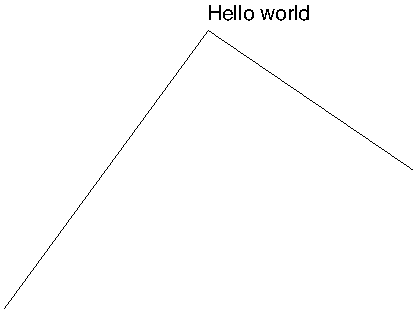
\includegraphics[width=200pt]{directuse-eg}
\end{minipage}

\end{centering}
\medskip

  
\end{document}
